\subsection{Farey cascade to the singular parameter $\alpha_1^*$ for $\rho=1/\pi$}\label{app:pi-cascade}

For $K{=}N{=}2$ at $\psi=0.4\pi$, $\alpha_0=1$, the rotation number $\rho(\alpha_1)$ traces a complete devil's staircase (Section~\ref{sec:bifurcation}).
Irrational $\rho$ are achieved on a measure-zero set; we locate the singular $\alpha_1^*$ realizing $\rho=1/\pi$ by walking a Farey cascade of rational plateaus toward it.
The continued-fraction expansion of $1/\pi$ is $[0;3,7,15,1,292,\ldots]$, so the convergents are $1/3,7/22,106/333,113/355$, with semi-convergents $(7m{+}1)/(22m{+}3)$ filling the path from $7/22$ to $106/333$ as $m=1,\ldots,15$.

\paragraph{Method.}
For any rational $\rho=p/q$ with $\gcd(p,q)=1$, the unique balanced firing word is the mechanical Sturmian
$\sigma_{p/q}=(s_0,\ldots,s_{q-1})$ with $s_k=\lfloor(k{+}1)p/q\rfloor-\lfloor kp/q\rfloor\in\{0,1\}$.
Building the $2\times 2$ symbolic return matrix
$\vv{M}_\sigma(\alpha_1)=\prod_{k=q-1}^{0}\vv{M}_{s_{k+1}\leftarrow s_k}(\alpha_1)$ in $300$-digit \texttt{mpmath} and dehomogenizing its dominant eigenvector gives the predicted orbit $(\xi_0,\ldots,\xi_{q-1})$.
The orbit is realized iff the admissibility margin
\begin{equation}\label{eq:cascade-margin}
m(\alpha_1)\;=\;\min_{k}\Bigl(c_{s_{k+1}}-\!\!\max_{j\ne s_{k+1}}c_j\Bigr)
\end{equation}
is positive at the predicted orbit, where the decay factors $c_j=\alpha_j/(\DD_j^\top\yy_k^+)$ are evaluated at each post-spike readout~$\yy_k^+$. The plateau is then $\{\alpha_1:m(\alpha_1)>0\}$.

We bisect both edges of each plateau in turn, walking down the Farey chain:
the left bracket at level $(p_n,q_n)$ is the precisely refined right edge of $7/22$,
\[\alpha_1^{(7/22)\mathrm{R}}=0.5223343802940303852301165223341492397534560143394308644640508665058751\ldots\] (computed first at \texttt{mpmath} $\textsf{dps}=300$), and the right bracket is the previous level's left edge.

\begin{figure}[h]
\centering
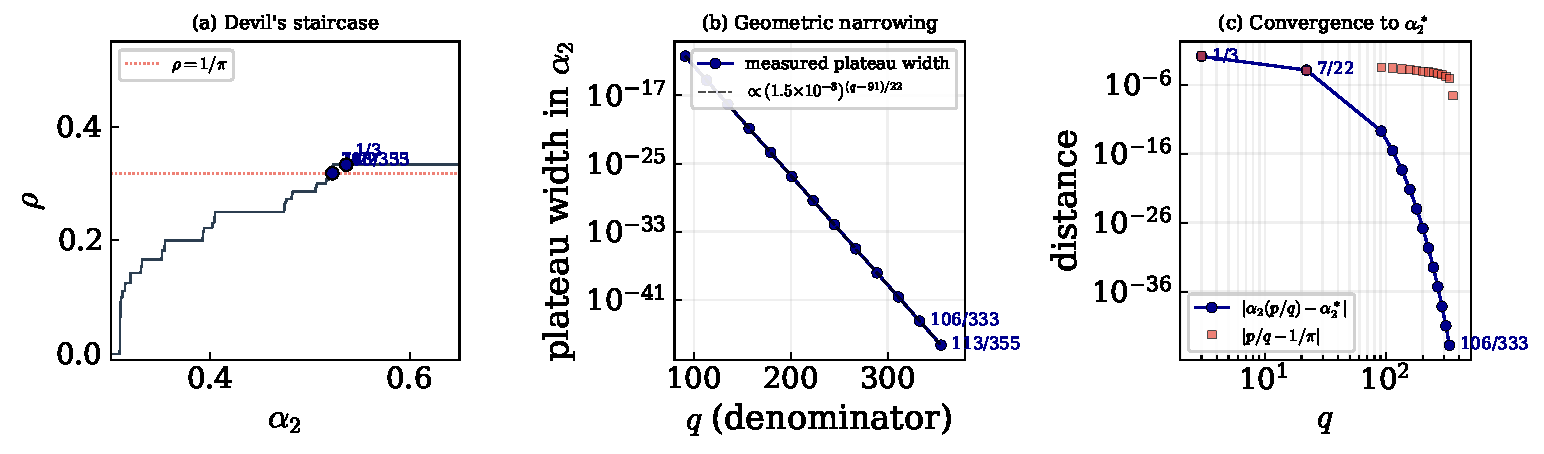
\includegraphics[width=0.95\textwidth]{figures/pi_approximants.pdf}
\caption{Farey cascade toward $\rho=1/\pi$. \textbf{(a)}~The devil's staircase with the four continued-fraction convergents marked. \textbf{(b)}~Plateau widths in $\alpha_1$ along the Farey chain decay geometrically by ${\sim}1.5\times 10^{-3}$ per step of $q$ by $22$. \textbf{(c)}~The plateau centres' distance to the cascade limit $\alpha_1^*$, alongside $|p/q-1/\pi|$ for comparison; both follow the same super-polynomial convergence.}
\label{fig:pi_approximants}
\end{figure}

\paragraph{Results.}
The 13~plateaus from $29/91$ down to the convergent $113/355$ all admit positive-width plateaus of unambiguously detectable width (Table~\ref{tab:cascade}, Figure~\ref{fig:pi_approximants}). Plateau widths decay geometrically by a factor of $\approx 1.5\times 10^{-3}$ per Farey step (each step adds $22$ to $q$), so the convergent $113/355$ has plateau width $4.95\times 10^{-47}$ in $\alpha_1$, far below the $10^{-16}$ double-precision floor that defeats simulation-based searches.

\begin{table}[h]
\centering
\begin{tabular}{rcc}
\hline
$\rho=p/q$ & $q$ & plateau width \\
\hline
$29/91$    &  91 & $3.99\times 10^{-13}$ \\
$36/113$   & 113 & $5.96\times 10^{-16}$ \\
$43/135$   & 135 & $8.91\times 10^{-19}$ \\
$50/157$   & 157 & $1.33\times 10^{-21}$ \\
$57/179$   & 179 & $1.99\times 10^{-24}$ \\
$64/201$   & 201 & $2.97\times 10^{-27}$ \\
$71/223$   & 223 & $4.45\times 10^{-30}$ \\
$78/245$   & 245 & $6.64\times 10^{-33}$ \\
$85/267$   & 267 & $9.93\times 10^{-36}$ \\
$92/289$   & 289 & $1.48\times 10^{-38}$ \\
$99/311$   & 311 & $2.22\times 10^{-41}$ \\
$106/333$  & 333 & $3.32\times 10^{-44}$ \\
$113/355$  & 355 & $4.95\times 10^{-47}$ \\
\hline
\end{tabular}
\caption{Plateau widths along the Farey cascade toward $\rho=1/\pi$, computed in \texttt{mpmath} at $300$-digit precision. Each step from $q$ to $q{+}22$ shrinks the plateau by ${\sim}1.5\times 10^{-3}$.}
\label{tab:cascade}
\end{table}

\paragraph{The singular point.}
Along the cascade, the right edge of $113/355$ and the left edge of $106/333$ coincide to all $\sim 80$~digits resolved in our run, giving the cascade limit
\begin{equation}
\alpha_1^*\;\approx\;0.522334380294030385230116522334149239753456014389052084833331820664863883\ldots
\end{equation}
This is the unique $\alpha_1$ at which the SCN has rotation number exactly $1/\pi$: the firing word is the aperiodic Sturmian $\sigma_{1/\pi}$ and the orbit closure has empty interior on $\Bsp_0$.

\paragraph{Irrational firing ratios are realized; finite-precision simulation only sees rational ones.}
The rotation number $\rho(\alpha_1)$ is continuous and monotone non-decreasing in $\alpha_1$ on this family (Section~\ref{sec:bifurcation}; \citealp{herman1979conjugaison}). It takes the value $0$ at small $\alpha_1$ and rises through $1/2$ at large $\alpha_1$. By the intermediate value theorem, $\rho$ attains \emph{every} real value in $[0,1/2]$ --- every rational, every algebraic and transcendental irrational --- so for each target $\omega\in[0,1/2]$ there exists $\alpha_1^*(\omega)$ realizing it.\footnote{Uniqueness up to plateau interior: for rational $\omega=p/q$, all $\alpha_1$ in the plateau realize $\omega$; for irrational $\omega$ the realization is at a single point.} Rational $\omega$ are realized on plateaus of positive Lebesgue measure; irrational $\omega$ are realized at single points forming a Cantor-like measure-zero set. The dynamics at every $\alpha_1$ is well defined --- deterministic update law, real-valued state, Birkhoff average converging to $\rho(\alpha_1)$ --- including at every irrational realization. What finite-precision simulation cannot do is \emph{set} $\alpha_1$ to a singular value: a double-precision $\alpha_1$ lies within $10^{-16}$ of its representable neighbour, and the plateaus have full Lebesgue measure in any region of the staircase, so round-off lands on a rational. Reaching $\alpha_1^*(1/\pi)$ requires the Farey cascade --- approaching the singular parameter from a sequence of computable rational neighbours at extended precision.

\paragraph{The cascade is the theory.}
$\alpha_1^*$ has no known closed-form expression --- the cascade itself is the canonical characterization. Three equivalent definitions all reduce to the same infinite procedure.

\emph{(i) As an inverse rotation number.} $\alpha_1^*$ is uniquely defined by $\rho(\alpha_1^*) = 1/\pi$, where the rotation number is the Birkhoff limit
\[
\rho(\alpha_1) \;=\; \lim_{n\to\infty} \frac{1}{n}\sum_{k=0}^{n-1} \mathbf{1}_{\{\text{neuron 1 fires at step } k\}}.
\]
Inverting a Birkhoff limit is itself an infinite procedure: $\alpha_1^*$ is a limit of limits.

\emph{(ii) As a topological conjugacy.} The natural rigidity statement is \textbf{Denjoy's theorem} \citep{denjoy1932courbes}: \emph{every orientation-preserving $C^2$ diffeomorphism $F$ of the circle with irrational rotation number $\rho$ is topologically conjugate to the rigid rotation $R_\rho(x)=x+\rho\pmod 1$ --- that is, there exists an orientation-preserving homeomorphism $h$ of the circle with $h\circ F\circ h^{-1}=R_\rho$} (see also \citealp{herman1979conjugaison}). The conjugacy is at most $C^0$, not analytic. Applied at $\alpha_1^*$ (rotation number $1/\pi$) it would give $F_{\alpha_1^*}$ conjugate to $R_{1/\pi}$. Two caveats. First, the SCN return map is continuous and piecewise M\"obius but only $C^0$ at the partition point $\xi_{\mathrm{part}}$, so the $C^2$ hypothesis of the classical theorem fails. Piecewise-smooth extensions \citep{liousse2005nombre} restore the conclusion provided no break point lies on the orbit closure; we do not verify this condition for the SCN, and record it as the natural sufficient hypothesis under which $\alpha_1^*$ corresponds to dynamics genuinely conjugate to rotation rather than to a Denjoy counter-example with a Cantor-set attractor. Second, in either case the conjugacy $h$ is at most $C^0$ and has no known closed-form expression, so it provides no analytic shortcut to $\alpha_1^*$.

\emph{(iii) As a constant defined by an infinite cascade.} A clean analogue is the \textbf{Feigenbaum bifurcation constant} of period-doubling: for a one-parameter family $f_r$ with a quadratic maximum (e.g.~the logistic map $f_r(x)=rx(1-x)$), let $r_1<r_2<\cdots$ be the parameter values at successive period-doubling bifurcations on the route to chaos. The ratio
\[
\delta \;=\; \lim_{n\to\infty}\frac{r_n-r_{n-1}}{r_{n+1}-r_n} \;\approx\; 4.66920160910299\ldots
\]
is a specific real number defined entirely by this limit and is universal across families with quadratic maxima \citep{feigenbaum1978quantitative}. No closed form is known for $\delta$; it is computable to arbitrary precision only by walking the cascade. Our $\alpha_1^*(1/\pi)$ is of the same character: a specific real number defined by an infinite Farey cascade, with no known closed form, computable only by walking the cascade to the required depth. Each Farey level here adds ${\sim}\log_{10}(1.5{\times}10^{-3})^{-1}\approx 2.8$ digits of $\alpha_1^*$; stopping at $113/355$ gives the ${\sim}50$ verified digits reported above. The next CF convergent $33102/103993$ has plateau width $\sim 10^{-1\,400}$, beyond any feasible computation.
